\preClass{Coordinate Systems}



\noindent Watch the Pre-Class videos for Section 1.7 and answer the following questions. Remember that in your written work you are graded on the correctness of your supporting work and not just your final answer. Always give an exact answer unless you are explicitly told to round; calculator approximations will not receive full credit.

\begin{enumerate}

\item  Determine whether the function $f$ is even, odd, or neither.
 $$f(x)=4x^3-x$$


\vfill


\item  Evaluate the function for the given values of $x$.
\[
  f(x) =
  \begin{cases}
                                   x+3 & \text{for $x<-1$} \\
                                   x^2 & \text{for $-1 \leq x <2$}   \end{cases}
\]


\begin{enumerate}
\item $f(-2)=$\\
\item $f(-1)=$\\
\item $f(0)=$\\
\item $f(-5)=$\\


\end{enumerate}
\newpage

\item  Graph the piece-wise defined function.

\[
  f(x) =
  \begin{cases}
                                   2 & \text{for $x \leq -1$} \\
                                   2x & \text{for $x > -1$} 
                                     \end{cases}
\]


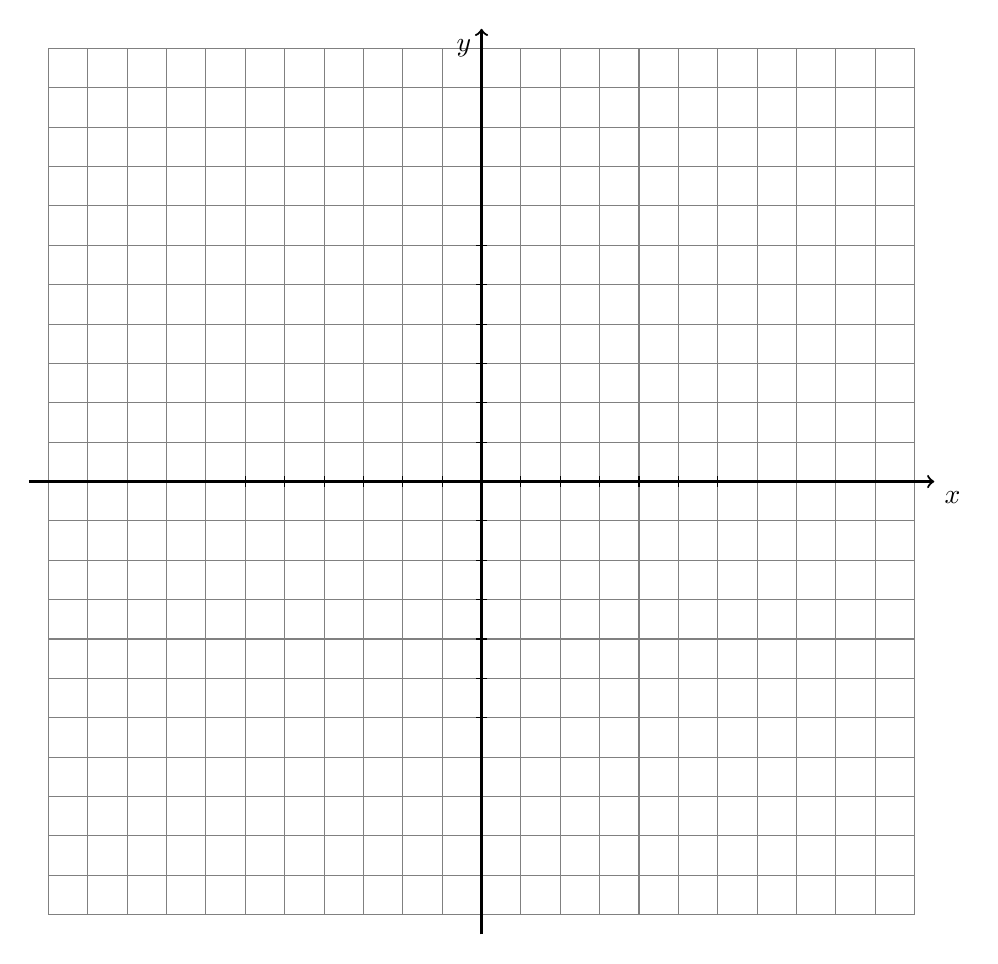
\begin{tikzpicture}[y=.5cm, x=0.5cm,font=\sffamily]
    %% ticks
    \draw[step = 1, gray] (-11,-11) grid (11,11);
    %% axis
    \draw[thick,->] (-11.5,0) -- coordinate (x axis mid) (11.5,0) node[anchor = north west] {$x$};
    \draw[thick,->] (0,-11.5) -- coordinate (y axis mid) (0,11.5) node[anchor = north east] {$y$};
    \foreach \y in {-6,-5,...,-1,1,2,...,6} {
      \draw (2pt, \y) -- (-2pt, \y);
    }
    \foreach \x in {-6,-5,...,-1,1,2,...,6} {
      \draw (\x,2pt) -- (\x,-2pt);
    }

  \end{tikzpicture}










\end{enumerate}


